\documentclass[11pt]{article}

\usepackage{sectsty}
\usepackage{graphicx}

\usepackage{svg}
\usepackage[off]{svg-extract}
\usepackage{relsize}
\usepackage{subcaption}
\usepackage{wrapfig}

\svgpath{{images}}

\usepackage{hyperref}
\usepackage{listings}
\usepackage{float}
\usepackage{booktabs}
\usepackage{makecell}

\usepackage{listings}
\usepackage{xcolor}

\definecolor{codegreen}{rgb}{0,0.6,0}
\definecolor{codegray}{rgb}{0.5,0.5,0.5}
\definecolor{codepurple}{rgb}{0.58,0,0.82}
\definecolor{backcolour}{rgb}{0.95,0.95,0.92}

\lstdefinestyle{mystyle}{
    backgroundcolor=\color{backcolour},   
    commentstyle=\color{codegreen},
    keywordstyle=\color{magenta},
    numberstyle=\tiny\color{codegray},
    stringstyle=\color{codepurple},
    basicstyle=\ttfamily\footnotesize,
    breakatwhitespace=false,         
    breaklines=true,                 
    captionpos=b,                    
    keepspaces=true,                 
    numbers=left,                    
    numbersep=5pt,                  
    showspaces=false,                
    showstringspaces=false,
    showtabs=false,                  
    tabsize=2
}
\lstset{style=mystyle}


% Margins
\topmargin=-0.45in
\evensidemargin=0in
\oddsidemargin=0in
\textwidth=6.5in
\textheight=9.0in
\headsep=0.25in

\def\rf{\emph{Risk Factor }}

\title{Project EE4C12 EPE ES}
\author{Benoît Jeanson \\ Employee 930283 \\ \href{mailto:b.jeanson@tudelft.nl}{b.jeanson@tudelft.nl}}

\date{\today}

\begin{document}
\maketitle
\pagebreak

% Optional TOC
% \tableofcontents
% \pagebreak

%--Paper--

\section{Summary}
    This project consists in designing machine learning models to assess the risk factor and corresponding risk state of a power grid (see Figure \ref{fig:grid}). The way the risk factor is determined is not known. Therefore, we use a statistical approach to evaluate it in contexts that are within the distribution of the training data. To this end, we follow the pipeline as depicted (see Figure \ref{fig:workflow}).
   
    \begin{wrapfigure}{R}{0.5\textwidth}
        \centering
        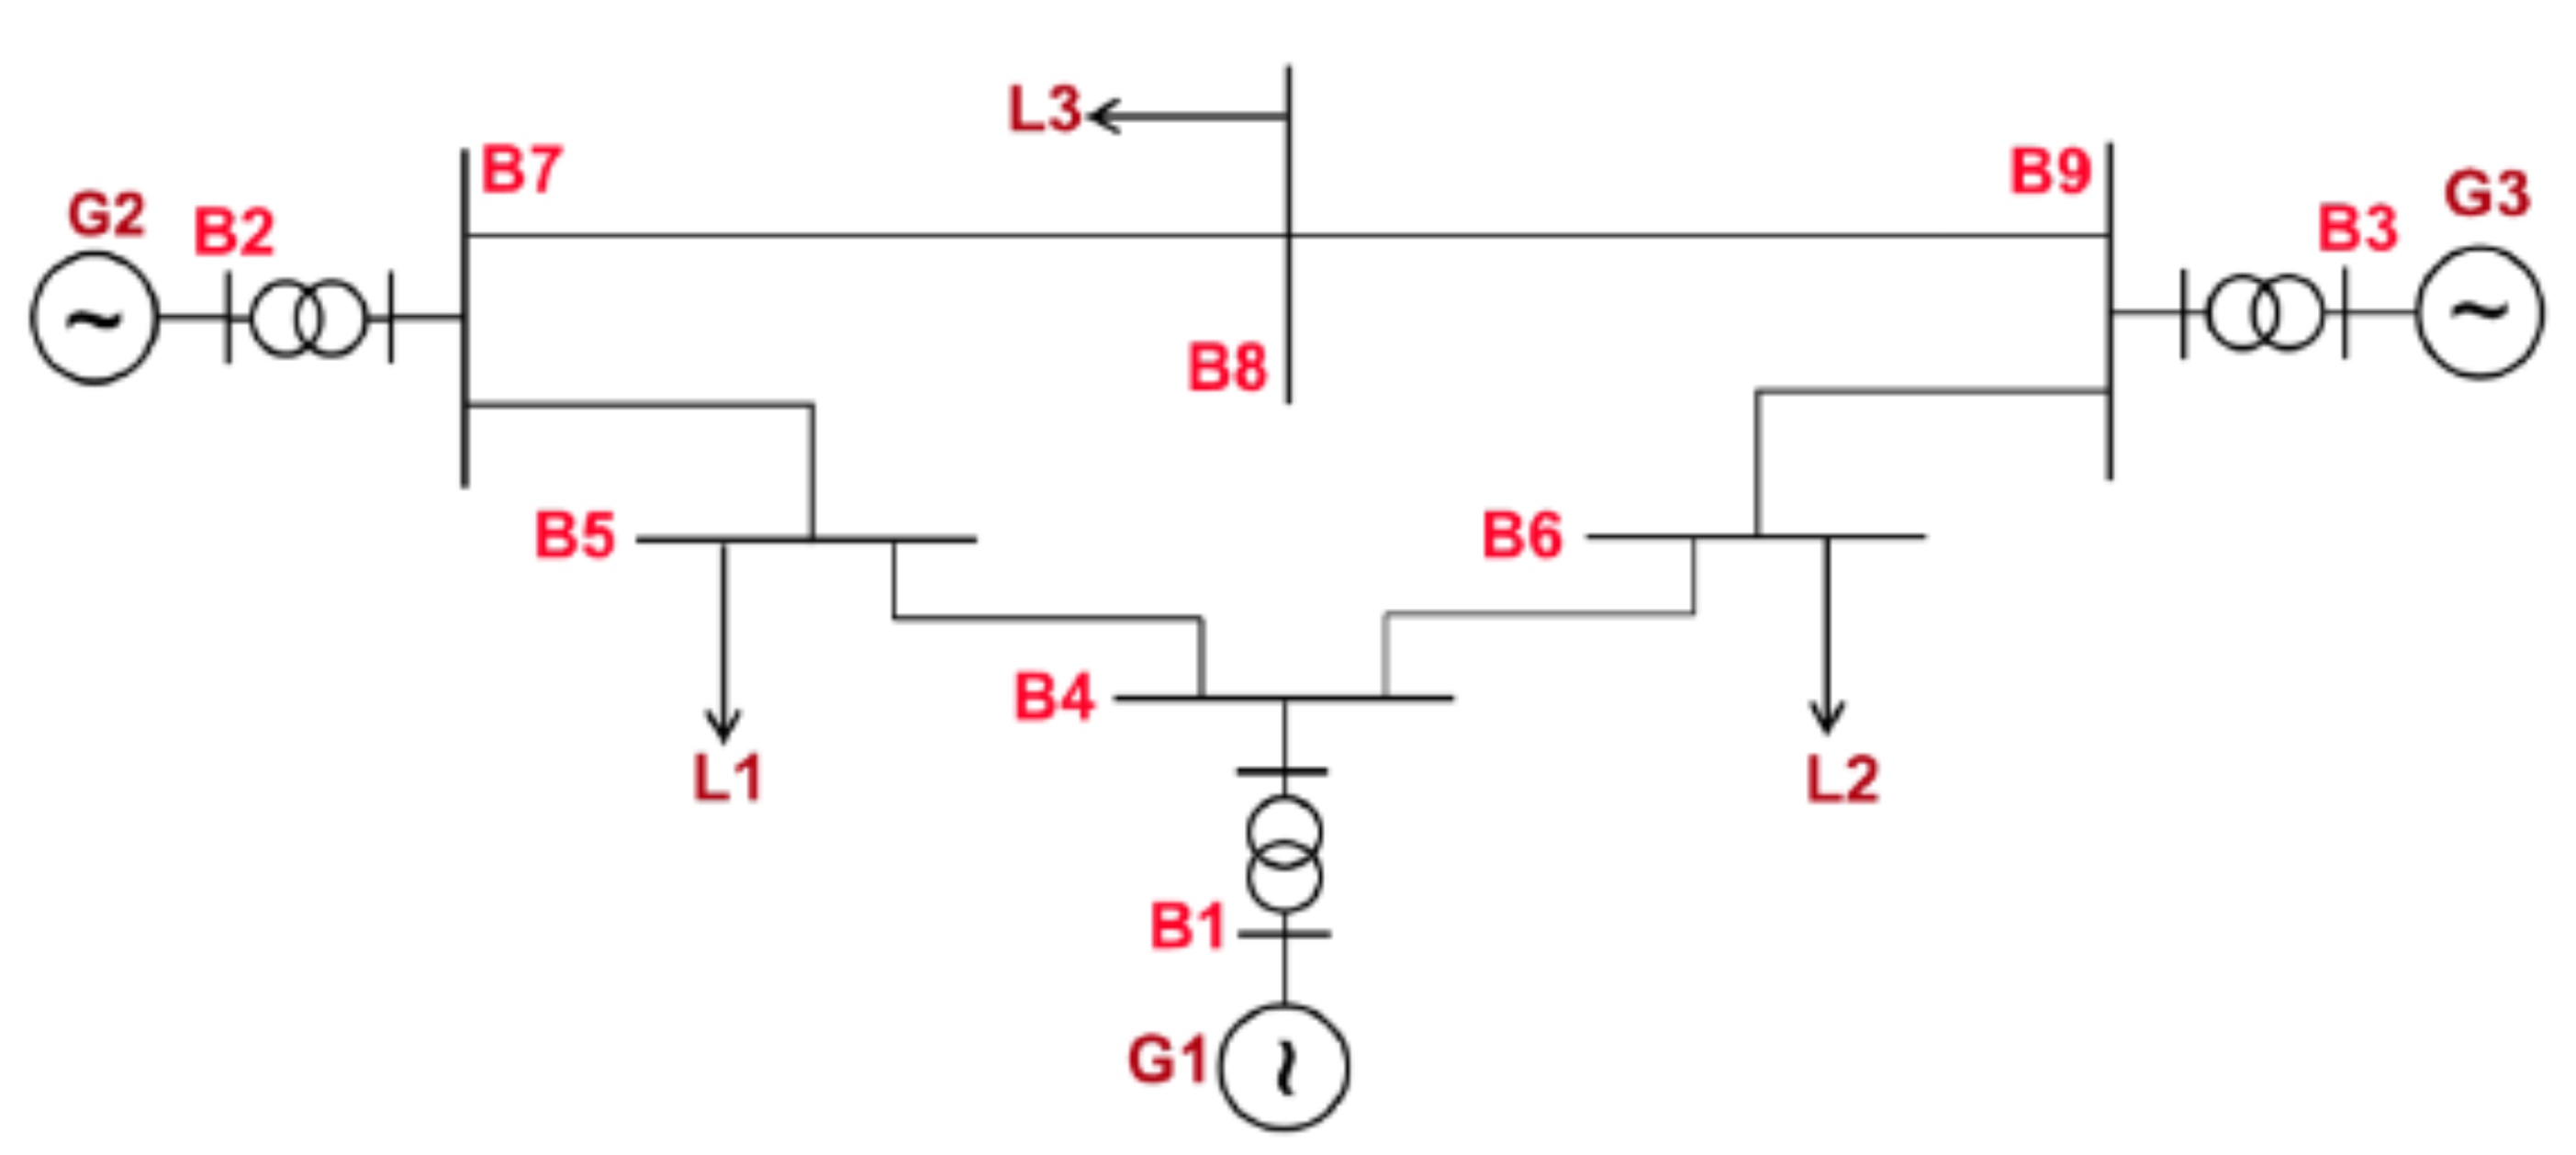
\includegraphics[scale=0.08]{images/IEEE9-grid.jpg}
        \caption{\label{fig:grid}9-buses power grid}
    \end{wrapfigure}

    This project report is structured according to the project description. The first part will describe the \emph{task 1} and consists in preparing the training: the data set is analyzed in order to identify what would be the relevant features to be used for the training process. The second part will describe the approach for the assessment of the \rf -- as a \emph{regression} problem. The third part will describe the approach for the assessment of the \emph{Risk State} -- as a \emph{classification} problem. A conclusion of the project implementation will then be proposed.

    All the simulations are performed using the python \emph{scikit-learn} framework, and run on a \emph{M1-chip MacBook Air}.

    \begin{figure}[h]
        \centering
        \includesvg[scale=0.5, pretex=\tiny]{images/pipeline.svg}
        \caption{\label{fig:workflow}Workflow of the approach}
    \end{figure}

    \pagebreak

\section{Task 1: preprocessing activities}
    %selected options, argumentation for the selection, model(s) developed, results, validation, comparisons.
    Before entering into any machine learning process, the input data has to be cleaned up and prepared. First as pointed out in the project statement, all combinations of 2 buses are provided in the initial data set -- including those combinations for which no line exists. In that case $P_{ij}=Q_{ij}=0$. We first remove all the rows that contains only zeros. This reduces the number of rows from 218 in the initial data set to 66. Then the output data \rf is extracted to properly isolate the input data (65 remaining rows) and the output one.

    The next step consists in analyzing each remaining feature to identify if they are relevant for training. Some data can be misleading, some others are proportional to one another, which could impede the training because of the collinearity of features.  

    First, we proceed to an analysis of the \emph{demand}. By plotting ${Pd}_i$ and ${Qd}_i$ for i in $\{5, 6, 8\}$ (e.g. Figure \ref{demandPQ} for demand-5) we can identify:
    \begin{itemize}
        \item For each $i$, ${Qd}_i$ looks proportional to ${Pd}_i$, which suggests a fixed $tan{\varphi}={{Qd}_i}/{{Pd}_i}$. The amplitudes of $tan{\varphi}$ values throughout all the samples being lower than $10^{-7}$ confirms that observation. Therefore, it is not necessary to keep both $P$ and $Q$ as they provide the same information.
        \item The demands are correlated per time slots of 1000 samples -- which becomes obvious with figure \ref{Pd_6-8vs5}. This observation is actually not useful for the training since the generation time series patterns are not correlated to the demand ones.
    \end{itemize}
    
    
    \begin{figure}[H]
        \begin{subfigure}[t]{.4\textwidth}
            \centering
            \includesvg[scale=0.75, pretex=\tiny]{demandPQ}
            \subcaption{\label{demandPQ}$P$ and $Q$ for demand-5 -- which suggests proportionality.}
        \end{subfigure}\hspace{0.1\textwidth}
        \begin{subfigure}[t]{.4\textwidth}
            \centering
            \includesvg[scale=0.75, pretex=\tiny]{Pd_6-8vs5}
            \subcaption{\label{Pd_6-8vs5}Ratio of $P$ for demand 6 and 8 vs 5 -- demands are proportional by piece of 1000 samples.}
        \end{subfigure}
        \caption{\label{Demand}Demand related curves}
    \end{figure}


    Regarding the \emph{generation} plan: the data set provides the active power $P$ for the 3 units: $\{1, 2, 3\}$, and $Q$ values only for units 2 and 3.
    \begin{itemize}
        \item Generation-1 is the \emph{slack} node. Indeed, the voltage is perfectly sustained at $1.3 p.u.$. Moreover, when comparing the ${Pg}_1$ with ${Pflow}_{1-4}$, one can see (figure \ref{Pslack}) that the output flow (on the line) differs from ${Pg}_1$ -- which shows that ${Pg}_1$ is the generation command value and not the generation output.
        \item The voltage can also be considered steady for generation 2 and 3 with amplitudes lower than $10^{-5}p.u.$
        \item As for the demand, the $tan{\varphi}$ look steady for generation 2 and 3, which would contradict the previous point as it is impossible in an evolving context to sustain both voltage and reactive power at the same time. Figure \ref{QGen2} shows that actually, the $Q$ value given is actually not followed: this is certainly the time series of the command that would be followed if the generator had been in \emph{P, Q} mode -- which is not the case. The $Q$ values for the generators shall not be used. They would actually not mislead the models -- as the model does not rely the physics -- this would only be redundant information with $P$ time series.
        \item The $P$ flows of Generation 2 and 3 follow their respective commands (e.g. Figure \ref{PGen2}).
    \end{itemize}
    Thus, we can conclude the $P,Q$ data provided for the generators, as well as the voltages on their connected buses, are useless as redundant with the data provided for their output flows are physically more relevant and better help in understanding the \emph{'Risk Factor'}.
    
    \begin{figure}[H]
        \begin{subfigure}[t]{.27\textwidth}
            \centering
            \includesvg[scale=0.75, pretex=\tiny]{PFlow1-4vsPgen1}
            \subcaption{\label{Pslack}$P$ Generation-1: output vs command value: the generator does not follow the command, it is actually the slack node.}
        \end{subfigure}\hspace{0.1\textwidth}
        \begin{subfigure}[t]{.27\textwidth}
            \centering
            \includesvg[scale=0.75, pretex=\tiny]{QGene2vsFlow}
            \subcaption{\label{QGen2}$Q$ Generation-2: output vs command value: the generator is in \emph{P, V} mode and does not follow the command.}
        \end{subfigure}\hspace{0.1\textwidth}
        \begin{subfigure}[t]{.27\textwidth}
            \centering
            \includesvg[scale=0.75, pretex=\tiny]{PGene2vsFlow}
            \subcaption{\label{PGen2}$P$ Generation-2: output vs command value: the flow follows the command.}
        \end{subfigure} 
        \caption{\label{Generation} Generation related curves}
    \end{figure}

    
    Regarding the \emph{voltage}, one can point out that all the information on the state of a power system is embedded in the \emph{voltage angles} and \emph{magnitudes} at each bus. Therefore, in theory, the \rf could be deduced using only the voltage data. However, in practice, as the equations connecting the various physical values to the voltage are nonlinear, leveraging other intermediate physical values (i.e. between the voltage and the Risk Factor) in the design of the models improves the results. Plotting the various curves of the voltage brings these observations: the voltage magnitudes on the generation buses that are steady -- and will not be used -- and the voltage profiles are evolving presenting regularities similar to the risk factor profile.

    Regarding the \emph{branches}, $P$ and $Q$ values are given on both sides of each. The active power (Figure \ref{fig:Pbranch}) on both sides are similar (few losses), while the reactive power behavior (Figure \ref{fig:Qbranch}) between both sides is much more volatile  -- except for the branches that are directly connecting generation buses, which are probably short and are of low impedance.
        
    \begin{figure}[H]
        \begin{subfigure}[t]{.4\textwidth}
            \centering
            \includesvg[scale=0.75, pretex=\tiny]{Pbranch5-7}
            \subcaption{\label{fig:Pbranch}$P$ Branch 5-7 vs 7-5}
        \end{subfigure}\hspace{0.1\textwidth}
        \begin{subfigure}[t]{.4\textwidth}
            \centering
            \includesvg[scale=0.75, pretex=\tiny]{Qbranch5-7}
            \subcaption{\label{fig:Qbranch}$Q$ Branch 5-7 vs 7-5}
        \end{subfigure}
        \caption{\label{fig:Branch} Branches related curves}
    \end{figure}

    Based on that investigation, the features that are candidates for the training are: the voltage magnitudes of all buses except those of the generators, the voltage angles of all nodes except for \emph{bus-1} which is the slack node, the active flows of the branches connected to buses hosting a generator, all the reactive flows on branches, the active power of the demand, and -- probably useless, to be tested -- one active power per branch. The efficiency of the learning could be further investigated trough various combinations of these features.

    \pagebreak

\section{Task 2: Estimation of the risk factor \emph{R}}
    To identify the risk factor, simulations were made with various set of features -- according the recommendations of Task 1. 6 combinations (Table \ref{tab:featureCombinations}) of features were tested with 3 kinds of model: a regression tree, a linear regression, and a neural network -- MLP -- (Table \ref{tab:modelsReg}). The first two were only tested with the default parameters whereas latest was tested with various parameters.
    
    \begin{table}[h]
        \centering
        \begin{tabular}{@{}cl@{}}
            \toprule
                \textbf{Set} & \textbf{Features} \\
            \midrule
                A & Voltage angles and magnitudes \\
                B & $(P,Q)$ flows on generators \\
                C & Voltage angles and magnitudes, $(P,Q)$ flows on generators \\
                D & Voltage angles and magnitudes, $P$ flows on generators, all $Q$ flows \\
                E & Voltage angles and magnitudes, $P$ flows on generators, all $Q$ flows, $P$ demands \\
                F & Voltage angles and magnitudes, $P$ flows on generators, all $Q$ flows, $P$ demands, $P$ flows direct \\
            \bottomrule
        \end{tabular}
        \caption{Features combinations set}
        \label{tab:featureCombinations}
    \end{table}
    
    Note that, \emph{voltage magnitudes} only concern buses that do not have generation, and that \emph{voltage angles} are for all the buses except \emph{bus-1}, \emph{$(P,Q)$ flows on generators} are taken from the branch that is connecting the corresponding generator, and \emph{$P$ flows direct} are taken on one side of each branch.

    \begin{table}[h]
        \centering
        \begin{tabular}{lll}
            \toprule
            \textbf{Model} & \textbf{Paramètres} \\
            \midrule
            TreeRegression  & default \\ \hline
            LinearRegression  & default \\  \hline
            MLP &
            \begin{tabular}[]{ll}
                hidden\_layer\_sizes & (100, 100), (100, 100, 100), (100, 100, 100, 100)\\ \hline
                alpha & 0.01, 0.1\\ \hline
                max\_iter & 300, 500, 1000
            \end{tabular} \\
            \bottomrule
        \end{tabular}
        \caption{Tested regression models and their parameters}
        \label{tab:modelsReg}
    \end{table}

    A systematic grid search is performed among the combinations of features and all the models and parameters. This was done 3 times which highlighted the influence of the random seed for the \emph{MLP} model. The table \ref{tab:best5rg} shows the results for the 5 best combinations of features and model parameters. In this top-5, the results are very close. Moreover, regarding the fact that they are ranked in different orders from one training to another, we will consider them equivalent. The only model remaining is \emph{MLP} with $Alpha=0.1$, the number of max iterations has no visible influence, and the architecture with 3 or 4 layers have similar results. Regarding the features combinations, $D$, $E$ and $F$ are equally represented, therefore, $D$ contains all the information needed to asses the \rf.

    \begin{table}[h]
        \centering
        \begin{tabular}{cclcccccc}
            \toprule
                Training & Group & Layers & Alpha & max\_iter & MSE ($\times 10^{-3}$) & R2 & Training Time \\
            \midrule
                1 & D & (100, 100, 100, 100) & 0.1 & 300 & 2.32 & 0.976 & 10s \\
                & F & (100, 100, 100) & 0.1 & 300 & 2.37 & 0.975 & 6s \\
                & D & (100, 100, 100, 100) & 0.1 & 500 & 2.42 & 0.975 & 9s \\
                & E & (100, 100, 100, 100) & 0.1 & 300 & 2.44 & 0.975 & 7s \\
                & D & (100, 100, 100) & 0.1 & 500 & 2.47 & 0.974 & 8s \\
            \hline
                2 & E & (100, 100, 100) & 0.1 & 1000 & 2.35 & 0.975 & 5s \\
                & D & (100, 100, 100, 100) & 0.1 & 1000 & 2.37 & 0.975 & 5s \\
                & F & (100, 100, 100, 100) & 0.1 & 500 & 2.41 & 0.975 & 8s \\
                & F & (100, 100, 100, 100) & 0.1 & 300 & 2.42 & 0.975 & 7s \\
                & E & (100, 100, 100) & 0.1 & 500 & 2.42 & 0.975 & 4s \\
            \hline
                3 & E & (100, 100, 100, 100) & 0.1 & 1000 & 2.34 & 0.976 & 4s \\
                & F & (100, 100, 100, 100) & 0.1 & 300 & 2.35 & 0.975 & 13s \\
                & D & (100, 100, 100, 100) & 0.1 & 500 & 2.36 & 0.975 & 8s \\
                & E & (100, 100, 100) & 0.1 & 300 & 2.37 & 0.975 & 4s \\
                & E & (100, 100, 100, 100) & 0.1 & 500 & 2.38 & 0.975 & 6s \\
            \bottomrule
        \end{tabular}
        \caption{The 5 best combinations of model parameters and features for 3 trainings}
        \label{tab:best5rg}
    \end{table}
    
    With the features set $D$, the results for the \emph{TreeRegression} are $MSE=7.79 \times 10^{-3}$ and $R2=0.920$, and for the \emph{LinearRegression}, $MSE=15.8 \times 10^{-3}$ and $R2=0.839$ -- both with training times around 100 ms. These results show that, even if the MLP is outperforming them by almost one order of magnitudes on the $MSE$, these models are already very efficient, and have the merit of the simplicity. Regarding the $MLP$ parameters, once again \emph{max\_iter} has no influence on the performances of the training, whereas \emph{alpha} has a significant impact: all the training with a value of 0.01 have the worst performances ($MSE\simeq 4 \times 10^{-3}$ and $R2\simeq 0.95$). The 2 layers MLP have good performances, but remain below the MLP with 3 and 4 layers.

    The final test is then performed with the features set $D$, a \emph{4-layer MLP}, $max\_iter=1000$, and $Alpha=0.1$. On the test set, the results are $MSE=3.13 \times 10^{-3}$ and $R2=0.967$.

\pagebreak

\section{Task 3: Estimation of the risk state: \emph{Class}}
This part consist in estimating the \emph{Risk State}, which is function of the \rf according to the following thresholds:

$$ safe  < 0.1 \leq LowRisk < 0.35 \leq ModerateRisk < 0.7 \leq HighRisk $$

First, as a regressor was trained in the previous task, it can provide an easy first classifier, by assessing the risk factor of the situation and classify with the appropriate thresholds. The results are: accuracy: 0.84, precision: 0.83, recall: 0.85, F1: 0.84 and the confusion matrix: Figure \ref{fig:CM_rg}

\begin{figure}{}
    \centering
    \includesvg[scale=0.6, pretex=\tiny]{CM_rg}
    \caption{\label{fig:CM_rg}Confusion matrix with the regressor trained in task 2}
\end{figure}

Then, for this part, the intention was to test the function \texttt{RandomizedSearchCV} with \emph{SVC classifier}. Two sets of parameters were tested to assess the best set of parameters between \emph{SVC classifier} non-polynomial kernels (i.e. \emph{linear} and \emph{rbf}) that do not have the parameter \emph{degree} and the polynomial one.

\texttt{RandomizedSearchCV} was so stunning and easy to implement, it was worth testing it also with the \emph{MPLClassifier} which turned out to outperform the performances of the \emph{SVC} classifiers.

The results are in the Table \ref{tab:RandomizedSearchCV}

\begin{table}[h]
    \begin{tabular}{lccccccc}
        \toprule
        \textbf{Classifier} & \textbf{Param} & \textbf{Best} & \textbf{Accuracy} & \textbf{Precision} & \textbf{Recall} & \textbf{F1} \\
        \midrule
            \begin{tabular}{c}
                Non-Poly\\SVC         
            \end{tabular} &
            \begin{tabular}{l}
                C: \texttt{loguniform(1e-5, 1e2)} \\ kernel: 'linear', 'rbf'
            \end{tabular} & 
            \begin{tabular}{c}
                0.764\\'rbf        
            \end{tabular}
        & 0.854 & 0.852 & 0.855 & 0.853 \\
        \hline
        
        Poly SVC &
            \begin{tabular}{c}
                C: \texttt{loguniform(1e-5, 1e2)}\\degree: \texttt{np.arange(1, 5)}
            \end{tabular} &
            \begin{tabular}{c}
                18.636 \\ 2 
            \end{tabular} 
            & 0.818 & 0.821 & 0.819 & 0.819    \\
            
        \hline
        \begin{tabular}{c}
            MLP\\Classifier 
        \end{tabular}&
            \begin{tabular}{c}
                hls: (100, 100, 100) \\ (100, 100, 100, 100) \\ alpha:\\ \texttt{loguniform(1e-4, 1)} \\ activation:\\'logistic', 'tanh', 'relu'
            \end{tabular} &
            \begin{tabular}{c}
                (100, \\100, 100)\\ \\ 0.003 \\ \\  'logistic'
            \end{tabular}
            & 0.943 & 0.934 & 0.941 & 0.937 \\
        \bottomrule
    \end{tabular}
    \caption{parameters explored with \texttt{RandomsizedSearchCV} and results}
    \label{tab:RandomizedSearchCV}
\end{table}


\begin{figure}
    \centering
    \includesvg[scale=0.6, pretex=\tiny]{CM_classifier}
    \caption{\label{fig:CM_classifier}Confusion matrix with the \emph{MLPClassifier} trained in task 3}
\end{figure}

Out of curiosity, considering the excellent performances of the parameters identified for the \emph{MPLClassifier} by \texttt{RandomsizedSearchCV}, the parameters were tested to see if these parameters were also relevant for the regressor of task 2. The results are: $MSE = 4.70 \times 10^{-3}$ and $R2=0.951$, which does not outperform the previous models. Moreover, if the corresponding regressor is itself used for the classification, its performances (accuracy = 0.82) are poor compare to what was reached.

The final model is therefore the \emph{MPLClassifier} with the parameters identified by the random search. The confusion matrix is presented in Figure \ref{fig:CM_classifier}

\pagebreak

\section{Conclusion}

    This study on a small case turned out to be pretty complex and allows me exploring numerous aspects of the machine learning. Many options were not yet implemented that could have been very interesting. Regarding the preprocessing (task 1), the exploration could also include for example \emph{PCA} analysis to analyze the features through a more statistical approach. I preferred relying on my own experience of the domain -- which can be misleading: sometimes naive approaches turn out to be very fruitful. The work on the regressor (task 2) completed the analysis of the features by confirming a narrowed set of relevant features. The development of the grid search was done manually -- which gave a lot of control on the process and on the information retrieved. In task 3, I kept the features fine-tuned in task 2 and I could appreciate the power of \texttt{RandomsizedSearchCV} -- which is very efficient, especially allowing parallelization which significantly sped up the training. Mixing up the models and parameters between task 2 and 3  -- reuse of \emph{MLPRegressor} of task 2 for a classifier, use of the parameters identified in task 3 for a new regressor -- confirmed that principle that a model shall be trained as much as possible in strict accordance with its final usage.

\end{document}